\label{section:results}

\begin{table*}[t!]
\centering
\begin{tabular}{c|c|c|c|c|c|c|c|c|c|c}
        &         & Num       & Lines     &        &        & Potential & Validated  &         & Inj Time \\
Name    & Version & Src Files & C code    & N(DUA) & N(ATP) & Bugs      & Bugs       & Yield   & (sec)  \\\hline
file    & 5.22    & 19        & 10809     & 631    & 114    & 17518     & 774        & 39.0\%  & 16         \\  %    files verified.  sloc recomputed
%eog    & 3.4.2   &           & 22997     &        &        &           &            &         &         \\ 
readelf & 2.25    & 12        & 21052     & 3849   & 266    & 276367    & 1064       & 53.4 \% & 354     \\  % time verified.  files verified. sloc recomputed
bash    & 4.3     & 143       & 98871     & 3832   & 604    & 447645    & 192        & 9.5\%   & 153     \\  % time verified.  
tshark  & 1.8.2   & 1272      & 2186252   & 9853   & 1037   & 1240777   & 354        & 15.3\%  & 542     \\
\end{tabular} 
\caption{LAVA Injection results for open source programs of various sizes.
For each, a single input file was used to perform a taint analysis with PANDA.
Various program and dynamic trace statistics are reported as well as DUA, attack point (ATP), and yield (fraction of injected bugs that result in a segmentation violation).}
\label{table:insertion-results}
\end{table*}

%We evaluated LAVA in three ways.
We evaluated LAVA in two ways.
First, we injected large numbers of bugs into four open source programs: file, readelf (from binutils), bash, and tshark (command-line verison of Wireshark). %, and eog (aka Eye of GNOME, an image viewer).
For each of these, we report various statistics with respect to both the target program and also LAVA's success at injecting bugs.
Second, we evaluated the distribution and realism of LAVA's bugs by proposing and computing various measures.
%Third, we randomly sampled 20 injected bugs for each of these programs and used these to measure detection rates for two commercial and two open source bug finders.

\subsection*{Counting Bugs}

Before we delve into the results, we must specify what it is we mean by an injected bug, and what makes two injected bugs distinct. Although there are many possible ways to define a bug, we choose a definition that best fits our target use case: two bugs should be considered different if an automated tool would have to reasonabout them differently. For our purposes, we define a bug as a unique pair $(DUA, attack point)$. Expanding this out, that means that the source file, line number, and variable name of the DUA, and the source file and line number of the attack point must be unique.

Some might object that this artificially inflates the count of bugs injected into the program, for example because it would consider two bugs distinct if they differ in where the file input becomes available to the program, even if the same file input bytes are used in both cases. But in fact these should be counted as different bugs: the data and control flow leading up to the point where the DUA occurs will be very different, and vulnerability discovery tools will have to reason differently about the two cases.

\subsection{Injection Experiments}
\label{sec:results:subsec:injection}

The results of injecting bugs into open source programs are summarized in Table~\ref{table:insertion-results}.
In this table, programs are ordered by size, in lines of C code, as measured by David Wheeler's \verb+sloccount+.
A single input was used with each program to measure taint and find injectable bugs.
The input to \verb+file+ and \verb+readelf+ was the program \verb+ls+.
The input to \verb+tshark+ was a 16K packet capture file from a site hosting a number of such examples.  % [ http://www.stearns.org/toolscd/current/pcapfile/README.ethereal-pcap.html ]
%The input to \verb+eog+ was ... 
The input to \verb+bash+ was a 124-line shell script written by the authors.
% TRL -- removed this since table was too big and I wanted to add bug inj time
%The number of sequential and unique basic blocks in the PANDA trace for each program are reported as N(BBs) and N(BBu).
$N(DUA)$ and $N(ATP)$ are the number of DUAs and attack points collected by the FIB analysis.
Note that, in order for a DUA or attack point to be counted, it must have been deemed viable for some bug, as described in Section~\ref{sec:mining}.
The columns \emph{Potential Bugs} and \emph{Validated Bugs} in Table~\ref{table:insertion-results} give the numbers of both potential bugs found by FIB, but also those verified to actually return exitcodes indicating a buffer overflow (-11 for segfault or -6 for heap corruption) when run against the modified input.
The penultimate column in the table is \emph{Yield} which is the fraction of potential bugs what were tested and determined to be actual buffer overflows.
The last column gives the time required to test a single potential bug injection for the target.


Exhaustive testing was not possible; for each of the target programs, we attempted to validate 2000 potential bugs. 
Note that larger targets had larger numbers of potential bugs: \verb+tshark+ has over a million.
Larger targets also take longer to test: almost 10 minutes for \verb+tshark+.
This is because testing requires not only injecting a small amount of code to add the bug, but also recompiling and running the resulting program.
For many targets, we found the build to be subtly broken so that a \verb+make clean+ was necessary to pick up the bug injection reliably, which further increased testing time.

As the injected bug is designed to be triggered only if a particular set of four bytes in the input is set to a magic value, we tested with both the original input and with the modified one that contained the trigger. 
We did not encounter any situation in which the original input caused an overflow.


\begin{table}[b]
\centering
\begin{tabular}{l|l|l|l|l} 
       & \multicolumn{3}{c}{$mLIV$} &  \\  
$mTCN$ &         $[0,10)$ & $[10,100)$ & $[100,1000)$ & $[1000,+\inf]$ \\  \hline 
$[0,10)$ &       51.9\%   & 22.9\%     & 17.4\%       & 11.9\%          \\
$[10,100)$ &     --       & 0          & 0            & 0     \\
$[100,+\inf]$ &  --       & --         & --           & 0     \\ 
\end{tabular}
\caption{Yield as a function of both $mLIV$ and $mTCN$.  
Yield is highest for DUAs with low values for both of these measures, i.e., that are both a relatively uncomplicated function of input bytes and also that derive from input bytes involved in deciding fewer branches.
Cells for which there were no samples are indicated with the contents '--'.}
\label{table:yield-breakdown}
\end{table}

Yield varies considerably from less than 10\% to over 50\%.
To understand this better, we investigated the relationship between our two taint-based measures and yield.
For each DUA used to inject a bug, we determined $mTCN$, the maximum TCN for any of its bytes and $mLIV$, the maximum liveness for any label in any taint label set associated with one of its bytes.  
More informally, $mTCN$ represents how complicated a function of the input bytes a DUA is, and $mLIV$ is a measure of how much the control flow of a program is influenced by the input bytes that determine a DUA.
Table~\ref{table:yield-breakdown} is a two-dimensional histogram with the bins for $mTCN$ intervals along the vertical axis and bins for $mLIV$ along the horizontal axis.
The top-left cell of this table represents all bug injections for which $mTCN<10$ and $mLIV<10$, and the bottom-right cell is all those for which $mTCN>=1000$ and $mLIV>=1000$.
Recall that, when  $mTCN=mLIV=0$, the DUA is not only a direct copy of input bytes, but also, those input bytes have not been observed to be used in deciding any program branches. 
As either $mTCN$ or $mLIV$ increase, yield deteriorates.  
However, we were surprised to observe that $mLIV$ values of over 1000 still gave yield in the 10\% range.

\subsection{Bug Distribution}

It would appear as though LAVA can inject a very large number of bugs.  
If we extrapolate from yield numbers in Table~\ref{table:insertion-results}, we estimate there would be almost 400,000 real bugs if all were tested.

\noindent
But how well distributed is this set of bugs? 
For programs like \verb+file+ and \verb+bash+, between 11 and 44 source files  are involved in a potential bug.
In this case, the bugs appear to be fairly well distributed, as those numbers represent 58\% and 31\% of the total for each, respectively.
On the other hand, \verb+readelf+ and \verb+tshark+ fare worse, with only 2 and 122 source files found to involve a potential bug for each (16.7\% and 9.6\% of source files).
For \verb+tshark+, much of the code for which is devoted to parsing esoteric network protocols, coverage is probably the issue since we use only a single input.
Similiary, we only use a single hand-written script with \verb+bash+, with little attempt to cover a majority of language features.
We are unsure why so few of the source files in \verb+readelf+ involve a potential bug.
 

\subsection{Bug Realism}

\todo[inline]{Ricky: I think it would be particularly convincing to have a "case study" of an actual CVE that exhibits data flow properties similar to the kind of bug LAVA injects.  Or maybe a bug that adds unchecked tainted data to a pointer.} 

\begin{figure}
\centering
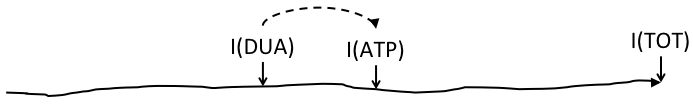
\includegraphics[width=3in]{trace-dua-atp.png}
\caption{A cartoon representing an entire program trace, annotated with instruction count at which DUA is siphoned off to be used, $I(DUA)$, attack point where it is used, $I(ATP)$, and total number of instructions in trace, $I(TOT)$.}
\label{fig:dua-atp-trace}
\end{figure}

The intended use of the bugs created by this system is as ground truth for development and evaluation of vulnerability discovery tools and techniques. 
Thus, it is crucial that they be realistic in some sense.  
Realism is, however, difficult to assess.

We examined three aspects of our injected bugs as measures of realism. 
The first two are DUA and attack point position within the program trace, which are depicted in Figure~\ref{fig:dua-atp-trace}.
That is, we determined the fraction of trace instructions executed at the point the DUA is siphoned off and at the point it is used to attack the program by corrupting an internal program value.
\todo[inline]{Ricky: what is the other "measures of realism?"  The "portion of hte trace between I(DUA) and I(ATP)? I(DUA)/I(ATP)? I(TOT)?} 

Histograms for these two quantities, $I(DUA)$ and $I(ATP)$, are provided in Figures~\ref{fig:dua-hist} and~\ref{fig:atp-hist}, where counts are for all potential bugs in the LAVA database for all five open source programs. 
DUAs and attack points are clearly available at all points during the trace, although there appear to be more at the beginning and end.
This is important, since bugs created using these DUAs have entirely realistic control and data-flow all the way up to $I(DUA)$.
Therefore, vulnerability discovery tools will have to reason correctly about all of the program up to $I(DUA)$ in order to correctly diagnose the bug.

The portion of the trace \emph{between} the $I(DUA)$ and $I(ATP)$ is of particular interest since LAVA currently makes data flow between DUA and attack point via a pair of function calls.
Thus, it might be argued that this is an unrealistic portion of the trace in terms of data flow.
The quantity $I(DUA)/I(ATP)$ will be close to 1 for injected bugs that minimize this source of unrealism.
This would correspond to the worked example in Figure~\ref{fig:worked-example}; the DUA is still in scope when, a few lines later in the same function, it can be used to corrupt a pointer.
No abnormal data flow is required.
The histogram in Figure~\ref{fig:rdf-hist} quantifies this effect for all potential LAVA bugs, and it is clear that a large fraction have $I(DUA)/I(ATP) \approx 1$, and are therefore highly realistic.

% Should we include some reasonable measure here where we don't turn out so well? Right now the evaluation feels kind of cooked -- we invent some measures and hey, LAVA looks really good under them! So we should a) acknowledge that it's not ideal that we're inventing our own metric for success, and b) we should maybe include something that seems like it would be a nice property, but that LAVA doesn't happen to have -- one that comes to mind is some measure of data flow complexity (rather than favoring flows that are "short" temporally)

\begin{figure}
\centering
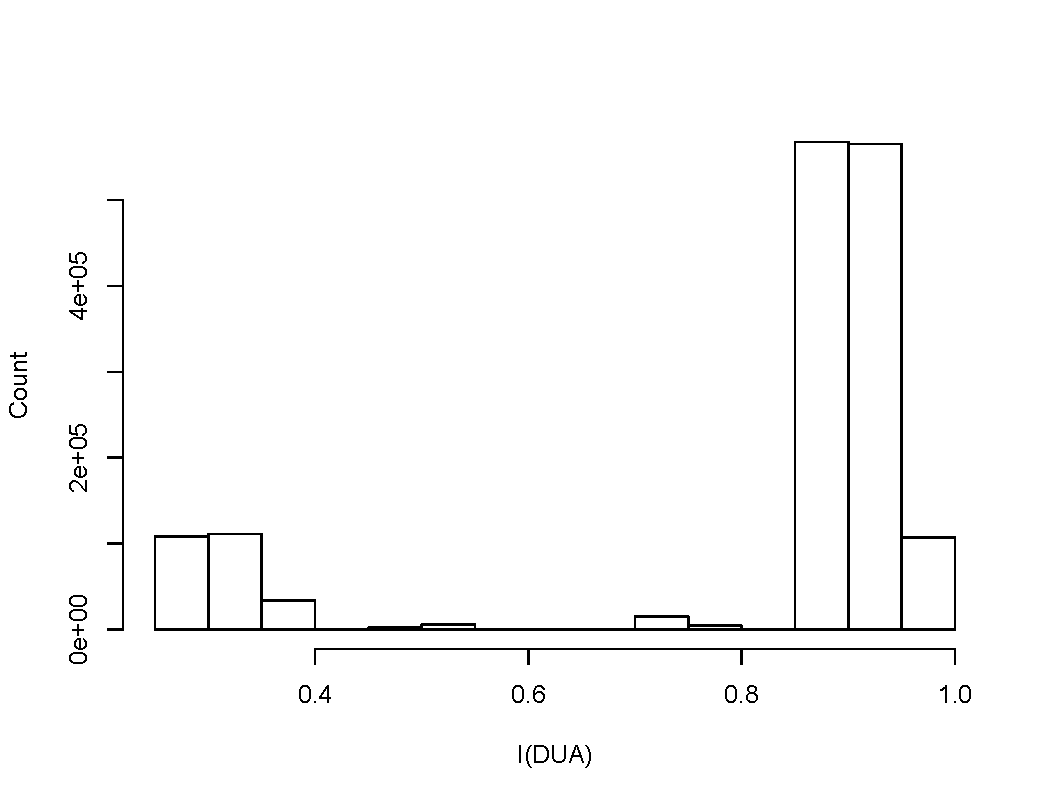
\includegraphics[width=3in]{dua.pdf}
\caption{Normalized DUA trace location}
\label{fig:dua-hist}
\end{figure}

\begin{figure}
\centering
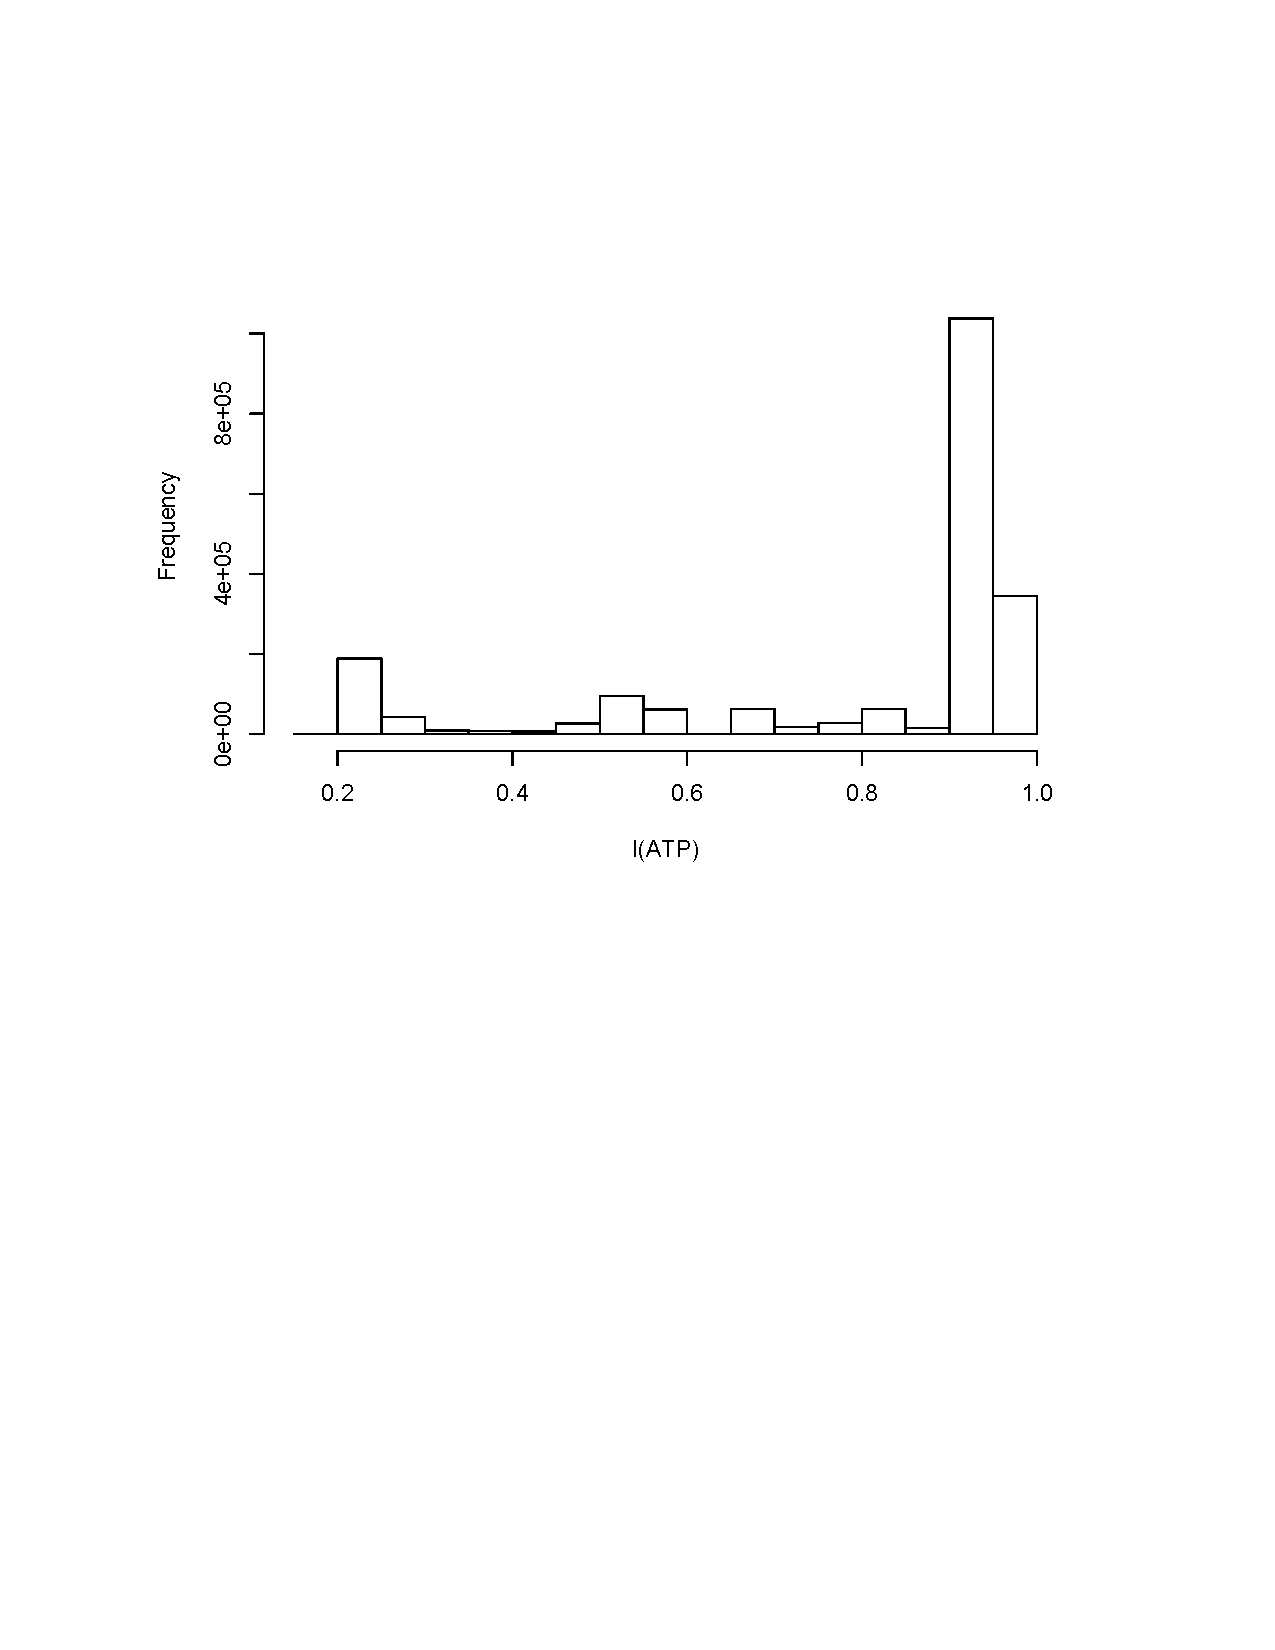
\includegraphics[width=3in]{atp.pdf}
\caption{Normalized ATP trace location}
\label{fig:atp-hist}
\end{figure}

\begin{figure}
\centering
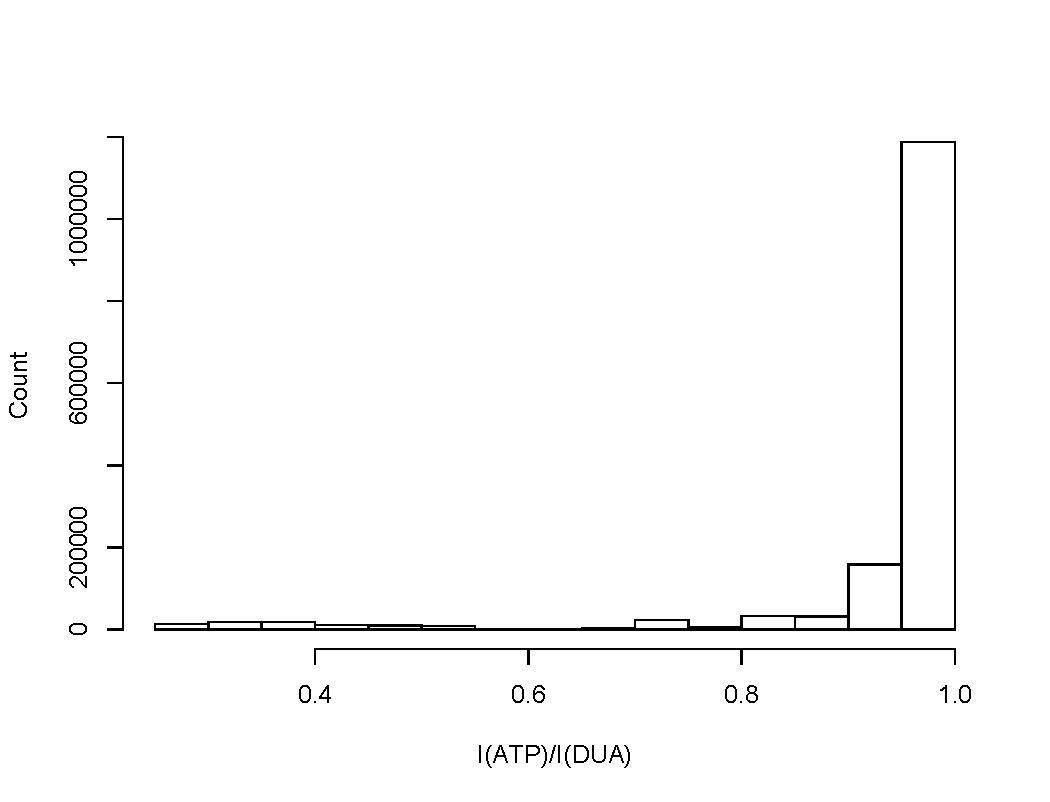
\includegraphics[width=3in]{rdf.pdf}
\caption{Fraction of trace with perfectly normal or realistic data flow, $I(DUA)/I(ATP)$}
\label{fig:rdf-hist}
\end{figure}




\subsection{Vulnerability Discovery Tool Evaluation}
We ran three vulnerability discovery tools on our corpora of bugs.
We chose an open source fuzzer, a Commericial Static Analyzer (CSE), and a Symbolic Execution and SAT Solver (SES) because they represented three unique approaches to vulnerability discovery.
Our corpora was a collection of 69 modifications of the program \verb+file+.
Each modification represented one of six different bug types and a randomly selected $Bug ID$.
All the tools were run on the same system, a x64 Debian 7 server with 16 cores at 3.50 GHz and 365 gB of \uppercase{ram}.
The tools were run to completion except in the case of the fuzzer where a wall time of 1 hour was given.
The evaluation results are summarized in Table~\ref{table:tool-eval-results}. 
\begin{table}[h]
\centering
\begin{tabular}{l|l|l|l|l|l|l} 
$Tool Type$ &                     \multicolumn{6}{|c}{$Bug Type$}                           \\  \hline  
            &                     \multicolumn{5}{|c|}{$Range Bug$}               & $KT$    \\   
            &    1       & $2^7$       & $2^{14}$     & $2^{21}$   & $2^{28}$     & 1   \\  \hline 
$Fuzzer$    &    0       & 0           & 0            & 7\%        & 58\%         & 0         \\
$CSA$       &    0       & 0           & 0            & 0          & 0            & 0         \\
$SES$       &    0       & 0           & 0            & 0          & 0            & 0         \\
\end{tabular}
\caption{Percentage of bugs found as a function of $Bug Type$ and $Tool Type$.  The most vulnerability finding tool proved to be the open source fuzzer.  However, it was only able to find bugs that had an enormous range of possible inputs to trigger the bug.}
\label{table:tool-eval-results}
\end{table}
%And something needs to go here when we get it from NEU who is doing the eval.



